%!TEX program = xelatex

\documentclass[a4paper, openany, oneside]{memoir}
\usepackage[no-math]{fontspec}
\usepackage{pgfplots}
\pgfplotsset{compat=newest}
\usepackage{commath}
\usepackage{mathtools}
\usepackage{amssymb}
\usepackage{amsthm}
\usepackage{booktabs}
\usepackage{mathtools}
\usepackage{xcolor}
\usepackage[separate-uncertainty=true, per-mode=symbol]{siunitx}
\usepackage[noabbrev, capitalize]{cleveref}
\usepackage{listings}
\usepackage[american inductor, european resistor]{circuitikz}
\usepackage{amsmath}
\usepackage{amsfonts}
\usepackage{ifxetex}
\usepackage[dutch,english]{babel}
\usepackage[backend=bibtexu,texencoding=utf8,bibencoding=utf8,style=ieee,sortlocale=en_GB,language=auto]{biblatex}
\usepackage[strict,autostyle]{csquotes}
\usepackage{parskip}
\usepackage{import}
\usepackage{standalone}
\usepackage{hyperref}
%\usepackage[toc,title,titletoc]{appendix}

\ifxetex{} % Fonts laden in het geval dat je met Xetex compiled
    \usepackage{fontspec}
    \defaultfontfeatures{Ligatures=TeX} % To support LaTeX quoting style
    \setromanfont{Palatino Linotype} % Tover ergens in Font mapje in root.
    \setmonofont{Source Code Pro}
\else % Terug val in standaard pdflatex tool chain. Geen ondersteuning voor OTT fonts
    \usepackage[T1]{fontenc}
    \usepackage[utf8]{inputenc}
\fi
\newcommand{\references}[1]{\begin{flushright}{#1}\end{flushright}}
\renewcommand{\vec}[1]{\boldsymbol{\mathbf{#1}}}
\newcommand{\uvec}[1]{\boldsymbol{\hat{\vec{#1}}}}
\newcommand{\mat}[1]{\boldsymbol{\mathbf{#1}}}
\newcommand{\fasor}[1]{\boldsymbol{\tilde{\vec{#1}}}}
\newcommand{\cmplx}[0]{\mathrm{j}}
\renewcommand{\Re}[0]{\operatorname{Re}}
\newcommand{\Cov}{\operatorname{Cov}}
\newcommand{\Var}{\operatorname{Var}}
\newcommand{\proj}{\operatorname{proj}}
\newcommand{\Perp}{\operatorname{perp}}
\newcommand{\col}{\operatorname{col}}
\newcommand{\rect}{\operatorname{rect}}
\newcommand{\sinc}{\operatorname{sinc}}
\newcommand{\IT}{\operatorname{IT}}
\newcommand{\F}{\mathcal{F}}

\newtheorem{definition}{Definition}
\newtheorem{theorem}{Theorem}


\DeclareSIUnit{\voltampere}{VA} %apparent power
\DeclareSIUnit{\pii}{\ensuremath{\pi}}

\hypersetup{%setup hyperlinks
    colorlinks,
    citecolor=black,
    filecolor=black,
    linkcolor=black,
    urlcolor=black
}

% Example boxes
\usepackage{fancybox}
\usepackage{framed}
\usepackage{adjustbox}
\newenvironment{simpages}%
{\AtBeginEnvironment{itemize}{\parskip=0pt\parsep=0pt\partopsep=0pt}
\def\FrameCommand{\fboxsep=.5\FrameSep\shadowbox}\MakeFramed{\FrameRestore}}%
{\endMakeFramed}

% Impulse train
\DeclareFontFamily{U}{wncy}{}
\DeclareFontShape{U}{wncy}{m}{n}{<->wncyr10}{}
\DeclareSymbolFont{mcy}{U}{wncy}{m}{n}
\DeclareMathSymbol{\Sha}{\mathord}{mcy}{"58}
\addbibresource{../../../../includes/bibliography.bib}

\begin{document}

\section{Derivation}
Consider the input signal to be a random stochastic process. Let the input signal be denoted by $x[n]$. Let the number of cosets by given by $M$. We denote the output of a coset $i$ by $y_i[n]$. To relate the output of a coset to the input signal, we need some mathematical constructs.

\subsection{Construction of the output of a coset}
In the chapter on sampling we have seen that every coset samples the input signal every $N$ samples. However, the cosets sample at different moments. To keep the way a coset samples the input signal as general as possible, we associate every coset $i$ to a signal $c_i[n]$ which specifies the way coset $i$ samples the input signal. Here $c_i[n] = 0$ for $n < 0$ and $n > N-1$. To illustrate the way $y_i[n]$, $x[n]$ and $c_i[n]$ are related, suppose that $N=4$. In this case \cref{fig:visualisation-yi} shows how $y_i[n]$ is related to $x[n]$ by $c_i[n]$. That is, every group of $N$ samples of the input signal yield one sample of the output of a coset. This is done by multiplying the samples in that group sample-wise by $c_i[N-1]$ to $c_i[0]$ and then summing them.
\begin{figure}
    \centering
    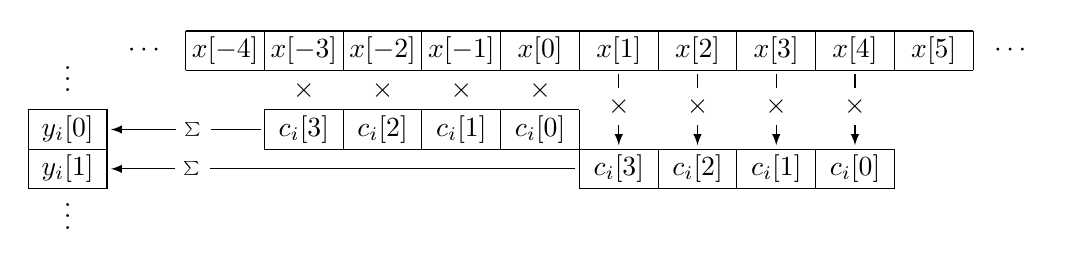
\begin{tikzpicture}
        \draw [black] (-5,0.5) -- (5,0.5);
        \draw [black] (-5,0) -- (5,0);

        \draw [black] (-4,-1) -- (0,-1);
        \draw [black] (-4,-0.5) -- (0,-0.5);
        \draw [black] (0,-1.5) -- (4,-1.5);
        \draw [black] (0,-1) -- (4,-1);
        \foreach \i in {-5,...,5} {
            \draw [black] (\i, 0) -- (\i, 0.5);
        }
        \foreach \i in {-4,...,5} {
            \draw ({\i-0.5},0.25) node[black] {$x[\i]$};
        }

        \foreach \i in {-4,...,0} {
            \draw [black] (\i, -0.5) -- (\i, -1);
        }
        \foreach \i in {0,...,3} {
            \draw ({(3-\i)-3.5},-0.75) node[black] {$c_i[\i]$};
        }

        \foreach \i in {0,...,4} {
            \draw [black] (\i, -1.5) -- (\i, -1);
        }
        \foreach \i in {0,...,3} {
            \draw ({(3-\i)+0.5},-1.25) node[black] {$c_i[\i]$};
        }

        \foreach \i in {-4,...,-1} {
            \draw (\i+0.5,-0.25) node {$\times$};
        }
        \foreach \i in {0,...,3} {
            \draw [black, >=latex, ->] (\i+0.5,-0.05)  -- node[pos=0.45,fill=white] {$\times$} (\i+0.5,-0.95);
        }

        \draw [black, >=latex, ->] (-4.05,-0.75) -- node[pos=0.45,fill=white] {\tiny$\sum$} (-5.95,-0.75);
        \draw [black, >=latex, ->] (-0.05,-1.25) -- node[pos=0.825,fill=white] {\tiny$\sum$} (-5.95,-1.25);
        \draw [black] (-7,-0.5) -- (-7,-1) -- (-6,-1) -- (-6,-0.5) -- (-7,-0.5);
        \draw [black] (-7,-1) -- (-7,-1.5) -- (-6,-1.5) -- (-6,-1) -- (-7,-1);
        \draw (-6.5,-0.75) node[black] {$y_i[0]$};
        \draw (-6.5,-1.25) node[black] {$y_i[1]$};
        \draw (-5.5,0.25) node {$\cdots$};
        \draw (5.5,0.25) node {$\cdots$};
        \draw (-6.5,-1.75) node {$\vdots$};
        \draw (-6.5,0) node {$\vdots$};
    \end{tikzpicture}
    \caption{Relationship between $y_i[n]$, $x[n]$ and $c_i[n]$ in the case that $N=4$}
    \label{fig:visualisation-yi}
\end{figure}
More mathematically,
\begin{align} \label{eq:yi}
    y_i[n]=\sum_{k=(n-1)N+1}^{nN} x[k]c_i[nN-k].
\end{align}
\Cref{eq:yi} precisely relates the output of coset $i$ to the input signal.

Consider the case that $c_i[n]=1$ for $n=S_i$ and otherwise zero. Then $y_i[n]$ consists of every $N-S_i$'th sample of every group of $N$ samples of $x[n]$. This is seen by substituting $c_i[n]$'s definition in \cref{eq:yi}, which yields that
\begin{align*}
    y_i[n]=\left.x[k]\right|_{nN-k=S_i}=x[nN-S_i].
\end{align*}
Notice that $y_i[n]$ is an $N$-decimation of the input signal. \cref{fig:visualisation-yi-example} illustrates this concept in the case that $N=4$ and $S_i=1$.
\begin{figure}
    \centering
    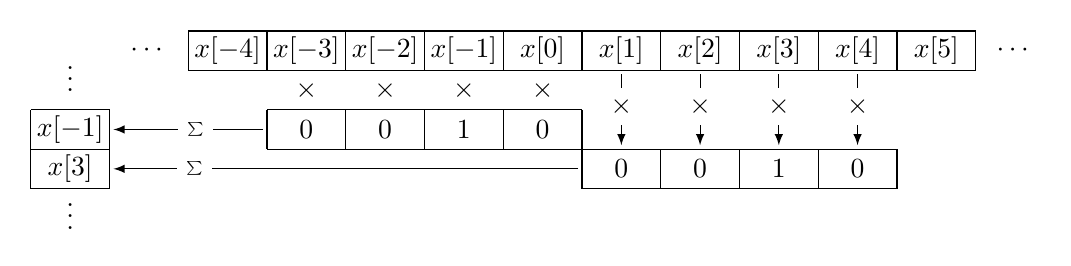
\begin{tikzpicture}
        \draw [black] (-5,0.5) -- (5,0.5);
        \draw [black] (-5,0) -- (5,0);

        \draw [black] (-4,-1) -- (0,-1);
        \draw [black] (-4,-0.5) -- (0,-0.5);
        \draw [black] (0,-1.5) -- (4,-1.5);
        \draw [black] (0,-1) -- (4,-1);
        \foreach \i in {-5,...,5} {
            \draw [black] (\i, 0) -- (\i, 0.5);
        }
        \foreach \i in {-4,...,5} {
            \draw ({\i-0.5},0.25) node[black] {$x[\i]$};
        }

        \foreach \i in {-4,...,0} {
            \draw [black] (\i, -0.5) -- (\i, -1);
        }
        \draw (-3.5, -0.75) node[black] {$0$};
        \draw (-2.5, -0.75) node[black] {$0$};
        \draw (-1.5, -0.75) node[black] {$1$};
        \draw (-0.5, -0.75) node[black] {$0$};

        \foreach \i in {0,...,4} {
            \draw [black] (\i, -1.5) -- (\i, -1);
        }
        \draw (0.5, -1.25) node[black] {$0$};
        \draw (1.5, -1.25) node[black] {$0$};
        \draw (2.5, -1.25) node[black] {$1$};
        \draw (3.5, -1.25) node[black] {$0$};


        \foreach \i in {-4,...,-1} {
            \draw (\i+0.5,-0.25) node {$\times$};
        }
        \foreach \i in {0,...,3} {
            \draw [black, >=latex, ->] (\i+0.5,-0.05)  -- node[pos=0.45,fill=white] {$\times$} (\i+0.5,-0.95);
        }

        \draw [black, >=latex, ->] (-4.05,-0.75) -- node[pos=0.45,fill=white] {\tiny$\sum$} (-5.95,-0.75);
        \draw [black, >=latex, ->] (-0.05,-1.25) -- node[pos=0.825,fill=white] {\tiny$\sum$} (-5.95,-1.25);
        \draw [black] (-7,-0.5) -- (-7,-1) -- (-6,-1) -- (-6,-0.5) -- (-7,-0.5);
        \draw [black] (-7,-1) -- (-7,-1.5) -- (-6,-1.5) -- (-6,-1) -- (-7,-1);
        \draw (-6.5,-0.75) node[black] {$x[-1]$};
        \draw (-6.5,-1.25) node[black] {$x[3]$};
        \draw (-5.5,0.25) node {$\cdots$};
        \draw (5.5,0.25) node {$\cdots$};
        \draw (-6.5,-1.75) node {$\vdots$};
        \draw (-6.5,0) node {$\vdots$};
    \end{tikzpicture}
    \caption{Relationship between $y_i[n]$, $x[n]$ and $c_i[n]$ in the case that $N=4$ and $c_i[n]=1$ for $n=1$ and otherwise zero}
    \label{fig:visualisation-yi-example}
\end{figure}

To analyse \cref{eq:yi}, we need a helper variable. Let
\begin{align*}
    z_i[n] = (c_i \ast x)[n]
\end{align*}
where $\ast$ denotes the convolution operator. The definition of the convolution operator yields that
\begin{align} \label{eq:zi}
    z_i[n] &= \sum_{k=\infty}^{\infty}x[k] c_i[n-k] \\
    &= \sum_{k=n-N+1}^{n} x[k] c_i[n-k],
\end{align}
since $c_i[n-k]=0$ for $k < n-N+1$ and $k > n$. \cref{fig:visualisation-zi} shows how $z_i[n]$, $x[n]$ and $c_i[n]$ are related in the case that $N=4$.
\begin{figure}
    \centering
    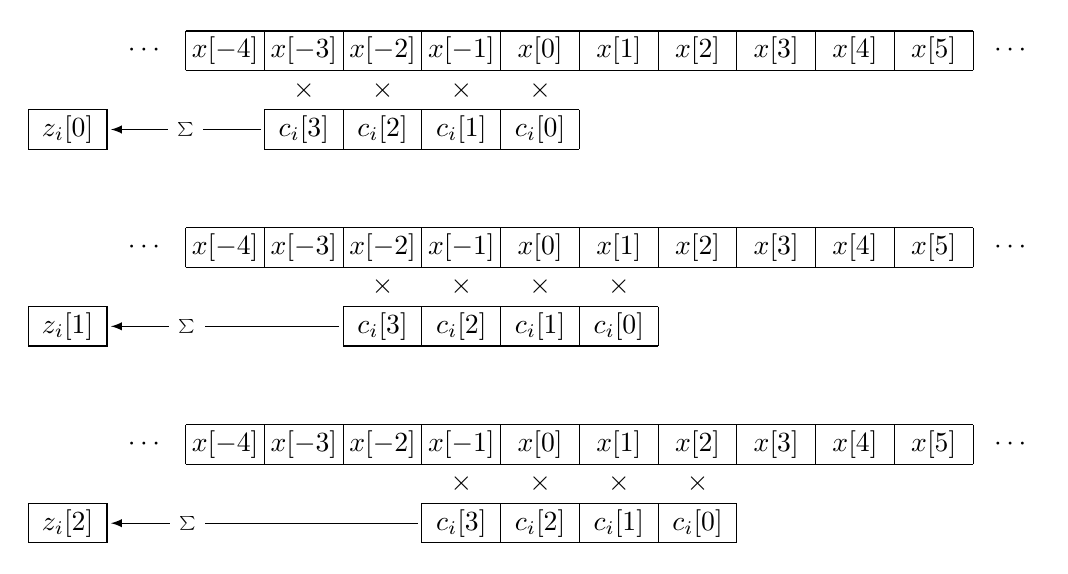
\begin{tikzpicture}
        \foreach \n in {0,1,2} {
            \begin{scope}[shift={(0,-2.5*\n)}]
                \draw [black] (-5,0.5) -- (5,0.5);
                \draw [black] (-5,0) -- (5,0);

                \draw [black] (-4+\n,-1) -- (0+\n,-1);
                \draw [black] (-4+\n,-0.5) -- (0+\n,-0.5);
                \foreach \i in {-5,...,5} {
                    \draw [black] (\i, 0) -- (\i, 0.5);
                }
                \foreach \i in {-4,...,5} {
                    \draw ({\i-0.5},0.25) node[black] {$x[\i]$};
                }

                \foreach \i in {-4,...,0} {
                    \draw [black] (\i+\n, -0.5) -- (\i+\n, -1);
                }
                \foreach \i in {0,...,3} {
                    \draw ({(3-\i)-3.5+\n},-0.75) node[black] {$c_i[\i]$};
                }

                \foreach \i in {-4,...,-1} {
                    \draw (\i+0.5+\n,-0.25) node {$\times$};
                }

                \draw [black, >=latex, ->] (-4.05+\n,-0.75) -- node[pos=(\n+1)/(2+\n),fill=white] {\tiny$\sum$} (-5.95,-0.75);
                \draw [black] (-7,-0.5) -- (-7,-1) -- (-6,-1) -- (-6,-0.5) -- (-7,-0.5);
                \draw (-6.5,-0.75) node[black] {$z_i[\n]$};
                \draw (-5.5,0.25) node {$\cdots$};
                \draw (5.5,0.25) node {$\cdots$};
            \end{scope}
        }
    \end{tikzpicture}
    \caption{Relationship between $z_i[n]$, $x[n]$ and $c_i[n]$ in the case that $N=4$}
    \label{fig:visualisation-zi}
\end{figure}
By inspection of \cref{eq:yi} and \cref{eq:zi}, we obtain that
\begin{align*}
    y_i[n]=z_i[nN].
\end{align*}


\subsection{Autocorrelation and cross-correlation}
The goal of the reconstruction method is to reconstruct the autocorrelation of the input signal given the output of all cosets. The autocorrelation of the input signal is given by
\begin{align*}
    r_x[n,m] = E(x[n]\conj{x}[n+m]).
\end{align*}
We assume that $x[n]$ is a wide sense stationary process. This means that $r_x[n,m]$ is independent of $n$. Therefore, we omit the $n$ in $r_x[n,m]$ and denote $r_x[n,m]=r_x[m]$. The cross-correlation of $z_i[n]$ and $z_j[n]$ is given by
\begin{align*}
    r_{z_i,z_j}[n,m]=E(z_i[n]\conj{z}_j[n+m]).
\end{align*}
Similarly, the cross-correlation of $y_i[n]$ and $y_j[n]$ is given by
\begin{align*}
    r_{y_i,y_j}[n,m]=E(y_i[n]\conj{y}_j[n+m]).
\end{align*}
Since the outputs of the cosets are assumed to be readily available, $r_{y_i,y_j}[n,m]$ can be determined. We plan to estimate $r_x[m]$ by making use of $r_{y_i,y_j}[n,m]$.

\subsection{Relating the autocorrelation of the input signal}

Since $x[n]$ is a wide sense stationary process, Theorem 11.5 of \cite{yates2005probability} yields that
\begin{align*}
    r_{z_i,z_j}[n,m] = (c_{i,j} \ast r_{x})[m]
\end{align*}
where
\begin{align} \label{eq:cij}
    c_{i,j}[m] = \sum_{k=-\infty}^{\infty}c_i[k] \conj{c}_j[k+m].
\end{align}
This shows that $r_{z_i,z_j}[n,m]$ is independent of $n$, we means we once more omit the $n$ in $r_{z_i,z_j}[n,m]$. Now the independence implies that
\begin{align*}
    r_{z_i,z_j}[mN] &= E(z_i[n]\conj{z}_j[n+mN]) \\
    &= E(z_i[nN]\conj{z}_j[nN+mN]) \\
    &= E(y_i[n]\conj{y}_j[n+m]) \\
    &= r_{y_i,y_j}[m],
\end{align*}
since we defined that $z_i[n]=y_i[nN]$. Therefore
\begin{align*}
    r_{y_i,y_j}[m] &= (c_{i,j}\ast r_{x})[mN].
\end{align*}
Consider \cref{eq:cij}. We know that $c_i[n]=0$ for $n < 0$ and $n > N-1$, which implies that $c_{i,j}[m]=0$ for $|m| > N-1$, since $c_i[k]\conj{c}_j[k+m]=0$ for $|m| > N-1$. So
\begin{align} \label{eq:ryiyj-rx}
    r_{y_i,y_j}[m] &= \sum_{k=-\infty}^{\infty}r_{x}[k]c_{i,j}[mN-k] \nonumber \\
    &= \sum_{k=(m-1)N+1}^{(m+1)N-1}r_{x}[k]c_{i,j}[mN-k].
\end{align}
This is the desired equation which relates the cross-correlation of the outputs of cosets $i$ and $j$ to the autocorrelation of the input signal. We see that every element of $r_{y_i,y_j}[m]$ depends on specific elements of $r_x[m]$ in a linear way. Consider the case that $N=3$. Then $c_{i,j}[m]=0$ for $|m| > 2$. \cref{fig:visualisation-ryiyj-rx} now illustrates the dependencies defined by \cref{eq:ryiyj-rx}.
\begin{figure}
    \centering
    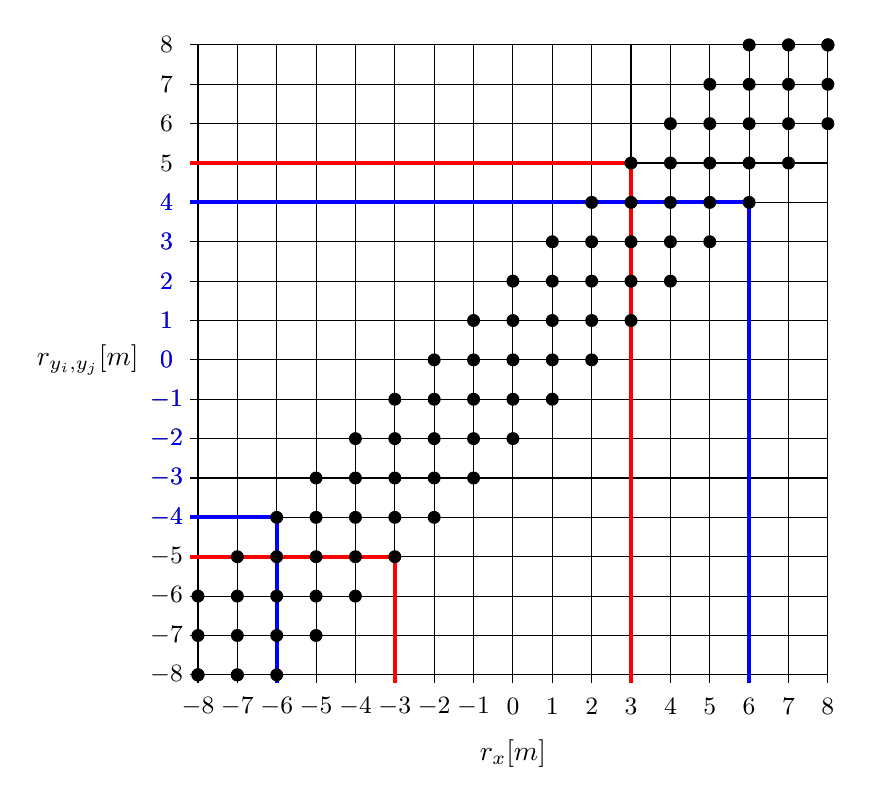
\begin{tikzpicture}
        \foreach \i in {-8,...,8} {
            \draw (-4.1,\i/2) -- (4, \i/2);
            \draw (\i/2, -4.1) -- (\i/2, 4);
            \draw (\i/2, -4.4) node {\small \num{\i}};
            \draw (-4.4, \i/2) node {\small \num{\i}};
        }

        % \foreach \i in {-6,...,6} {
        %     \draw (\i/2, -4.4) node[red] {\small \num{\i}};
        % }
        % \foreach \i in {-2,...,2} {
        %     \draw (\i/2, -4.4) node[blue] {\small \num{\i}};
        % }
        \foreach \i in {-4,...,4} {
            \draw (-4.4, \i/2) node[blue] {\small \num{\i}};
        }

        \draw [blue, thick, line width=1.5pt] (-4.1, -2) -- (-3, -2) -- (-3, -4.1);
        \draw [red, thick, line width=1.5pt] (-4.1, -2.5) -- (-1.5, -2.5) -- (-1.5, -4.1);
        \draw [blue, thick, line width=1.5pt] (-4.1, 2) -- (3, 2) -- (3, -4.1);
        \draw [red, thick, line width=1.5pt] (-4.1, 2.5) -- (1.5, 2.5) -- (1.5, -4.1);


        \foreach \i in {-2,...,2} {
            \foreach \j in {-8,...,8} {
                \draw [fill=black] (\j/2, {max(min(\i/2+\j/2, 4), -4)}) circle[radius=0.075,black];
            }
        }
        \draw (-5.4,0) node {$r_{y_i,y_j}[m]$};
        \draw (0,-5) node {$r_x[m]$};
    \end{tikzpicture}
    \caption{Illustration of the dependencies between the elements $r_{y_i,y_j}[m]$ and the elements of $r_x[m]$ introduced by \cref{eq:ryiyj-rx} in the case that $N=3$. The numbers at the axes represent the elements of the associated signal. A dot at the intersection of two lines represents a dependency between the associated elements. The coloured lines are used to discuss an example in \cref{subsec:estimating}.}
    \label{fig:visualisation-ryiyj-rx}
\end{figure}


\subsection{Estimating the autocorrelation of the input signal}
\label{subsec:estimating}
Before moving on in the derivation, we consider an example. Suppose that $N=3$. Also suppose that $r_{y_i,y_j}[m]$ is known for $|m| \le 4$. Furthermore, assume that $r_{y_i,y_j}[m]=0$ for $|m| \ge 5$. Since \cref{eq:ryiyj-rx} relates $r_{y_i,y_j}[m]$ to $r_x[m]$, we can use the known elements of $r_{y_i,y_j}[m]$ to solve for $r_x[m]$. In this example we investigate which elements of $r_x[m]$ can be solved for.

Again consider \cref{fig:visualisation-ryiyj-rx}. The known elements of $r_{y_i,y_j}[m]$ are depicted in blue. If we follow the blue lines, we can find out which elements of $r_x[m]$ are related to the known elements of $r_{y_i,y_j}[m]$. Therefore, the picture shows that given $r_{y_i,y_j}[m]$ for $|m| \le 4$, we should be able to solve $r_x[m]$ for $|m| \le 6$. However, we have to be careful, since we assumed that $r_{y_i,y_j}[m]=0$ for $|m| \ge 5$. If we follow the red lines, we find out that $r_{y_i,y_j}[m]=0$ for $|m| \ge 5$ implies that $r_x[m]$ can only be non-zero for $|m| \le 2$, since $r_{y_i,y_j}[m]$ would not zero for all $|m| \ge 5$ otherwise. Therefore, although we related $r_x[m]$ for $|m| \le 6$, we can only solve $r_x[m]$ for $|m| \le 2$.

We look at this problem in a more general way. Assume that $r_{y_i,y_j}[m]=0$ for $|m| > L$. Then observe that
\begin{align*}
    r_{y_i,y_j}[L+1] &= \sum_{k=LN+1}^{(L+1)N-1} r_x[k] c_{i,j}[k-(L+1)N].
\end{align*}
Since $c_{i,j}[m]$ is arbitrary, $r_{y_i,y_j}[L+1]=0$ implies that $r_x[m]=0$ for $LN+1 \le m \le (L+1)N-1$. Therefore, if we evaluate $r_{y_i,y_j}[m]=0$ for all $|m| > L$ in a similar way, then we obtain that $r_x[m]=0$ for $|m| > LN$.

Since $r_x[m]=0$ for $|m| > LN$, all that remains is estimating $r_x[m]$ for $|m| \le LN$. Aggregating \cref{eq:ryiyj-rx} for $|m| \le L$ yields that
\begin{align*}
    r_{y_i,y_j}[L] &= \sum_{k=(L-1)N+1}^{(L+1)N-1}r_{x}[k]c_{i,j}[LN-k] = \sum_{k=(L-1)N+1}^{LN}r_{x}[k]c_{i,j}[LN-k], \\
    r_{y_i,y_j}[L-1] &= \sum_{k=(L-2)N+1}^{LN-1}r_{x}[k]c_{i,j}[(L-1)N-k], \\
    &~~\vdots \\
    % r_{y_i,y_j}[0] &= \sum_{k=1-N}^{N-1}r_{x}[k]c_{i,j}[-k], \\
    % &~~\vdots \\
    r_{y_i,y_j}[-L+1] &= \sum_{k=-LN+1}^{(-L+2)N-1}r_{x}[k]c_{i,j}[(-L+1)N-k], \\
    r_{y_i,y_j}[-L] &= \sum_{k=(-L-1)N+1}^{(-L+1)N-1}r_{x}[k]c_{i,j}[-LN-k] = \sum_{k=-LN}^{(-L+1)N-1}r_{x}[k]c_{i,j}[-LN-k]. \\
\end{align*}
Here we used that $r_x[m]=0$ for $|m| > LN$ in reducing the limits of the sums in $r_{y_i,y_j}[L]$ and $r_{y_i,y_j}[-L]$. Although these equations look complicated, they can be written more compactly. To do this, let
\begin{align*}
    \vec{r}_x[k] =& \begin{bmatrix}
        r_x[(k+1)N-1] & \cdots & r_x[kN+1]
    \end{bmatrix}^T, \\
    \vec{c}^{-}_{i,j} =& \begin{bmatrix}
        c_{i,j}[-N+1] & \cdots & c_{i,j}[-1]
    \end{bmatrix} \text{ and } \\
    \vec{c}^{+}_{i,j} =& \begin{bmatrix}
        c_{i,j}[1] & \cdots & c_{i,j}[N-1]
    \end{bmatrix}.
\end{align*}
If we look carefully, we see that
\begin{align*}
    r_{y_i,y_j}[L] &= r_x[LN]c_{i,j}[0] + \sum_{k=(L-1)N+1}^{LN-1}r_x[k]c_{i,j}[LN-k] \\
    &=r_x[LN]c_{i,j}[0] + \vec{c}_{i,j}^+ \vec{r}_x[L-1].
\end{align*}
Similarly, we can write
\begin{align*}
    r_{y_i,y_j}[L-1] &= \vec{c}_{i,j}^{-} \vec{r}_x[L-1] + r_x[(L-1)N] c_{i,j}[0] + \vec{c}_{i,j}^{+} \vec{r}_x[L-2].
\end{align*}
The complicated system of equations now reduces to
\begin{align*}
    r_{y_i,y_j}[L] &= &&\hspace{12pt}r_x[LN] c_{i,j}[0] &&+ \vec{c}_{i,j}^+ \vec{r}_x[L-1] , \\
    r_{y_i,y_j}[L-1] &= \vec{c}_{i,j}^{-} \vec{r}_x[L-1] &&+ r_x[(L-1)N] c_{i,j}[0] &&+ \vec{c}_{i,j}^{+} \vec{r}_x[L-2], \\
    &~~\vdots \\
    r_{y_i,y_j}[-L+1] &= \vec{c}_{i,j}^{-}\vec{r}_x[-L+1] &&+ r_x[(-L+1)N] c_{i,j}[0] &&+ \vec{c}_{i,j}^{+}\vec{r}_x[-L], \\
    r_{y_i,y_j}[-L] &= \vec{c}_{i,j}^{-} \vec{r}_x[-L] &&+ r_x[-LN] c_{i,j}[0],
\end{align*}
which can be conveniently written as the matrix equation
\begin{align*}
    \begin{bmatrix}
        r_{y_i,y_j}[L] \\
        r_{y_i,y_j}[L-1] \\
        \vdots \\
        r_{y_i,y_j}[-L+1] \\
        r_{y_i,y_j}[-L]
    \end{bmatrix} = \begin{bmatrix}
        c_{i,j}[0] & \vec{c}^+_{i,j} \\
        \vec{c}^{-}_{i,j} & c_{i,j}[0] & \vec{c}^{+}_{i,j} \\
        % &\vec{c}^{-}_{i,j} & c_{i,j}[0] & \vec{c}^{+}_{i,j} \\
        &&\ddots \\
        &&\vec{c}^{-}_{i,j} & c_{i,j}[0] & \vec{c}^{+}_{i,j} \\
        &&&\vec{c}^{-}_{i,j} & c_{i,j}[0]
    \end{bmatrix} \begin{bmatrix}
        r_x[LN] \\
        r_x[LN-1] \\
        \vdots \\
        r_x[-LN+1] \\
        r_x[-LN]
    \end{bmatrix}.
\end{align*}
Denote the previous equation by
\begin{align} \label{eq:ryiyji-R-rx}
    \vec{r}_{y_i,y_j} = \mat{R}_{i,j} \vec{r}_x.
\end{align}
This equation relates the cross-correlation of the outputs of cosets $i$ and $j$ to the autocorrelation of the input signal. We can aggregate \cref{eq:ryiyji-R-rx} for all combinations of cosets. This yields that
\begin{align*}
    \begin{bmatrix}
        \vec{r}_{y_1,y_1} \\
        \vdots \\
        \vec{r}_{y_M,y_M}
    \end{bmatrix} = \begin{bmatrix}
        \mat{R}_{1,1} \\
        \vdots \\
        \mat{R}_{M,M}
    \end{bmatrix} \vec{r}_x.
\end{align*}
Denote the aggregation of \cref{eq:ryiyji-R-rx} by
\begin{align} \label{eq:ry-R-rx}
    \vec{r}_y = \mat{R} \vec{r}_x.
\end{align}
\Cref{eq:ry-R-rx} relates the cross-correlations of all combinations of outputs of cosets to the autocorrelation of the input signal. Note that $\mat{R}$ is an $M^2(2L+1) \times 2LN+1$ matrix. If $\mat{R}$ has full column-rank, then $\vec{r}_x$ can be solved for using least-squares, which involves solving the normal equations. These normal equations are given by
\begin{align} \label{eq:normal-rx}
    \mat{R}^T \vec{r}_y = \mat{R}^T \mat{R} \vec{r}_x.
\end{align}
We can use \cref{eq:normal-rx} to estimate the autocorrelation of the input signal if $\vec{r}_y$ is known. This concludes the estimation of the autocorrelation of the input signal.
\end{document}